\part{Termodinámica}

\vspace*{\fill}

\begin{center}
	\textit{La termodinámica es el estudio de las restricciones a las posibles propiedades de la materia que se derivan de las propiedades de simetría de las leyes fundamentales de la física.}
\end{center}

\vspace*{\fill}

\chapter{Conceptos Básicos}

\paragraph{Propósito: } La termodinámica busca describir sistemas de muchas partículas ($10^{23}$ típicamente). Gases, líquidos, cristales, estrellas, universo, \ldots ,  \underline{sistemas macroscópicos} y en particular, estudiar los procesos de transferencia de energía (trabajo y calor) entre cuerpos macroscópicos\footnote{Más adelante se tratará la parte microscópica con la Mecánica Estadística, poder explicativo y predictivo sobre propiedades macroscópicas de la materia, partiendo de una descripción microscópica.}. 

\begin{itemize}
	\item Definir cantidades físicas, "variables de estado" que caracterizan un sistema macroscópico: $V,T,N,U,\ldots$.
	\item Relacionar estas cantidades entre sí:
		\begin{enumerate}
			\item Válidas para cualquier sistema en equilibrio:
			\begin{enumerate}
				\item Leyes axiomáticas de la termodinámica, como Ley de la Energía, Ley de la Entroía, etc.
			\end{enumerate}
			\item Específicas
			\begin{enumerate}
				\item Por ecuaciones de estado como: fenomenológicas, empíricas, experimentales en la mayoria de los casos.
			\end{enumerate}
		\end{enumerate}
\end{itemize}


Es importante mencionar que la termodinámica clásica macroscópica no puede explicar porqué una ecuación de estado describe un sistema partícular.

\newpage

\section{Sistemas Termodinámicos y Cantidades de Estado}

\begin{enumerate}
	\item Sistema Termodinámico:
	\begin{figure}[H]
		\centering
		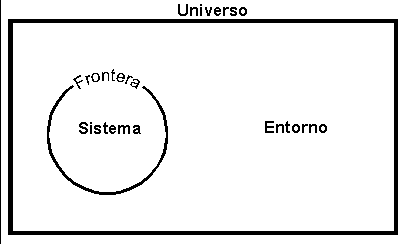
\includegraphics[scale=0.3]{./img/thermodynamicSystem.png}
		\label{thermodynamicSystem}
		\caption{Representación gráfica de las partes de un sistema termodinámico.}
	\end{figure}
	
	\item Tipos de Sistemas: (depende de la frontera)
	\begin{itemize}
		\item Sistemas aislados: No intercambian energía con el entorno. Los sistemas rígidos no pueden intercambiar trabajo y los adiabáticos no pueden intercambiar calor.
		\item Sistemas cerrados: Aquel que intercambia energía y trabajo con su entorno pero la masa permanece constante. Este intercambio de energía puede ser fluctuante aunque la caracterización de estas fluctuaciones no es de interes para la termodinámica.
		\item Sistemas abiertos: Aquel que intercambia tanto energía como materia con su entorno.
	\end{itemize}
	\item Variables de estado: Cualquier cantidad macroscópica que pueda describir el sistema. $E,V,N,T,P,S$, viscocidad $\mu$, composición química, etc. \textbf{no} $\{ \vec{r}_i , \vec{p} _i \}$. 
	\begin{itemize}
		\item Cantidades de estado extensivas: estas son aditivas (dependen de la cantidad de sustancia/moles o masa). Ejemplo: volumen, energía o entropía.
		\item Cantidades de estado intensivas: son independientes de la cantidad de sustancia del sistema, como la densiada, índice de refracción, presión o temperatura.
	\end{itemize}
\end{enumerate}



\section{Equilibrio y Temperatura (Ley Cero de la Termodinámica):}

\begin{enumerate}
	\item Estado de un sistema: Se define por un conjunto particular de \underline{valores} de sus variables termodinámicas.
	\begin{itemize}
		\item Como cada variable describe el sistema como un todo, en general son constantes en el espacio.
		\item Las variables pueden variar (lentamente en el tiempo).
	\end{itemize}
	\item Estado de equilibrio: cada variable tiene un único valor y este valor no cambia en el tiempo.
	\item Procesos cuasi-estáticos y no cuasi-estáticos: un proceso $\equiv$ un cambio de estado. (normalmente un proceso cuasi-estático se toma como un proceso reversible, aquí haremos una distinción). Un proceso no cuasi-estático puede ser una expansión muy rápida de un gas. Mientras que un proceso cuasi-estático puede ser reversible o irreversible como la expansión muy lenta de un gas con un pistón ($\delta V$ es muy pequeña). 
\end{enumerate}

\paragraph{Temperatura y Ley Cero: } La temperatura es una cantidad "desconocida" para la mecánica y electrodinámica, es una cantidad de estado especial para la termodinámica. Esta se define clásicametne mediante un proceso (\dsnote{no hay definición matemática...aún, se verá en la parte de mecánica estadística}). \\
La Ley Cero es una definición de la temperatura: Variable intensiva que es igual en dos sistemas en contacto, en equilibrio sin importar la forma y ubicación de este contacto. \\
Otra definición de la Ley Cero: "Cuando el contacto térmico entre A y B produce que B se caliente y A se enfríe, sin importar donde está este contacto, entonces no hay proceso que pueda calentar A y enfriar B que no induce un trabajo". \\

\" ESTADO DE EQUILIBRIO" $\neq$ \" ESTADO ESTACIONARIO", estar en equilibrio implica ser estado estacionario, pero no al contrario.


\section{Presión, Ecuación de Estado}
\begin{enumerate}
	\item Presión: En términos mecánicos es lo que ya se conoce $F/A$ y en términos microscópicos es la suma de las fuerzas que realizan todas las particulas del sistema sobre $A$.
	\item Ecuación de Estado: Relación entre variables independietes y la temperatura:
		$$ F (X,Y,T) = 0 $$
	\begin{figure}[H]
		\centering
		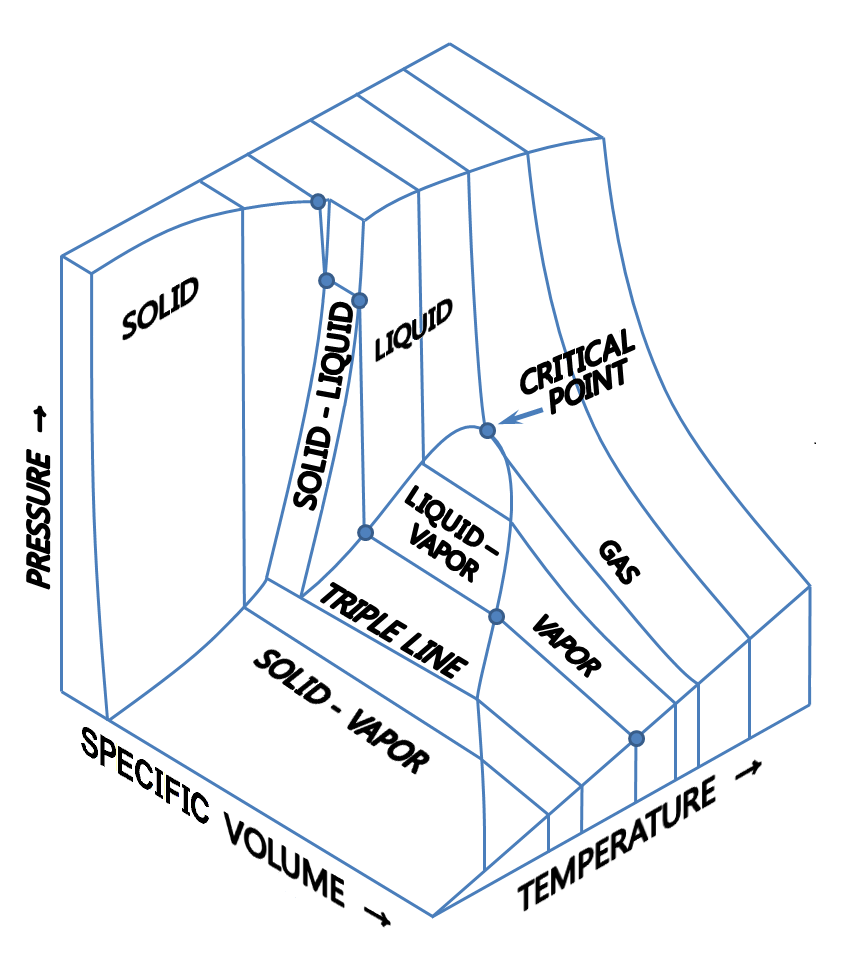
\includegraphics[scale=0.2]{./img/PVT_diagram.png}
		\label{PVT}
		\caption{Diagrama PVT.}
	\end{figure}
	Por ejemplo: Ecuación del gas ideal $pV = nRT$, la ecuación de gas real (expansión del Virial) $pV = Nk_B T + B(T) p + C(T) p^2 + \cdots$, donde $B(T), C(T), \ldots$ son los coeficientes del Virial o la de Van der Waals.
	\item Diferenciales Exactos (e Inexactos): Suponemos una ecuación de estado $z = f(x,y)$. Diferenciación $\dd{f(\vec{r})} = \vec{\nabla} f(\vec{r}) \cdot \dd{\vec{r}}$. $\dd{f}$ es un diferencial total si su integral no depende del contorno y solo de los extremos. Y este es exacto si $f$ es totalmente diferenciable, es decir, se pueden intercambiar las derivadas cruzadas (\dsnote{Básicamente, el teorema de Clairaut}). La implicación que esta tiene en termodinámica son las transformaciones reversibles (que pasan por estados de equilibrio), en estas la ecuación de estado el valor de las variables de estado es independiente del proceso que sigue para llegar a otro estado y esto es válido para cualquier variable de estado.
\end{enumerate}



\chapter{Primera Ley de la Termodinámia}


\section{Trabajo y Calor}
La energía total de un sistema puede variar si recibe (cede) trabajo o calor.

\begin{enumerate}
	\item Trabajo: Sistema sujeto a fuerzas externas. El sistema recibe energía durante una compresión. Con esta idea se tiene la convensión general (\dsnote{Bastante lógico}) $\delta W > 0$ si el sistema recibe trabajo y $\delta W < 0$ si el sistema realiza trabajo. \\
	Caso particular\footnote{Para más ejemplos ver p9 de \href{https://github.com/DSarceno/ExamenPrivado/blob/main/material_\%C3\%BAtil/termodinamica/Notas\%20Boyer.pdf}{Notas Boyer}} procesos cuasi-estáticos, $\dd{\vec{l}}$ es infinitesimal, es decir muy lento, entonces la aceleración del pistón es despresiable $\vec{F} _e + \vec{F}_i = 0$, donde $F_i$ es la fuerza ejercida por el sistema (fuerza interna) entonces $\delta W = - \vec{F} _i \cdot \dd{\vec{l}}$. Como el proceso es cuasi-estático, el sistema está en equilibrio $\leftarrow \, \exists$ presión en el sistema $\vec{F} _i = PA \vu{z}$. Reemplazando en la definición de trabajo $\delta W = -P\dd{V}$ ($P$ cantidad intensiva, $\dd{V}$ cantidad extensiva). \faExclamationTriangle $\,$ Durante el trabajo infinitesimal la presión es aproximadamente constante en el intervalo $[V,V + \dd{V}]$, pero si $\Delta V$ es grande, entonces
		$$ \Delta W = - \int _{V_1} ^{V_2} P(V) \dd{V}. $$
	\item Calor: Es una forma partícular de energía distinta al trabajo, por ejemplo en el calentamiento por entrega de calor no hay un trabajo visible. \\
	\textbf{Experimento de Joule: } Este fue crucial para demostrar la equivalencia entre trabajo mecánico y calor, sentando las bases de la primera Ley de la Termodinámica. 
	\begin{figure}[H]
		\centering
		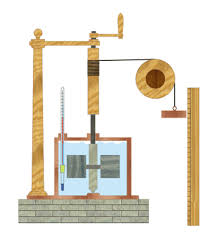
\includegraphics[scale=0.4]{./img/experimentoJoule.jpeg}
		\label{expJoule}
		\caption{Este consiste en un contenedor de agua aislado térmicamente, un sistema de paletas y un peso y una cuerda los cuales pasan por una polea.}
	\end{figure}
	El procedimiento es:
	\begin{enumerate}
		\item Elevación del peso: El peso se levanta a una cierta altura almacenando energía potencial gravitacional.
		\item Al liberar el peso, este desciende, la cuerda hace girar el eje el cual, a su vez, hace girar las paletas.
		\item Las paletas agitan el agua, creando fricción y generando calor.
	\end{enumerate}
	Joule encontró que el aumento de la temperatura del agua estaba directamente relacionado con la cantidad de trabajo mecánico realizado. Específicamente, pudo determinar la equivalencia entre unidades de trabajo (joules) y unidades de calor (calorías). La relación que encontró es aproximadamente $4.184$ joules por caloría. \\
	Joule demostró que el calor podía generarse mediante trabajo mecánico y viceversa, consolidado el concepto moderno de energía. \\
	Además podemos concluir que $\delta Q$ y $\delta W$ no son cantidades de estado, dependen del proceso, del camino ($Q$ y $W$ no son diferenciales exactos).
\end{enumerate}

\subsection{Naturaleza del Calor}
\" Energá distribuída de manera desordenada entre partículas. \" Es mucho más fácil convertir trabajo en calor que al revés. \\
Convensión: Misma que para el trabajo: $\delta Q = \delta Q_{\text{entorno} \leftarrow \text{ sistema}}$
\begin{itemize}
	\item $\delta Q > 0$ para un sistema que recibe calor del entorno.
	\item $\delta Q < 0$ para un sistema que cede calor al entorno.
\end{itemize}

\section{Energía Interna y Primera Ley}

\begin{enumerate}
	\item Energía interna: (definición microscópica) $U$ esta es la energía total del sistema, en el sentido mecánico-newtoniano, con  $N$ partículas
		$$ U = \sum _{i=1} ^N \frac{1}{2} m_i v_i ^2 + \sum _{i=1} ^N \sum _{j > i} ^N V(\vec{r}_i ,\vec{r}_j) + \sum _{i=1} ^N \vec{F} _e ^i \cdot \vec{r}_i . $$
	Donde se tiene la energía cinética, la potencial y las fuerzas externas. En general es imposible calcular esta energía y tampoco es el propósito de este curso. \dsnote{como siempre, a esperar a mecánica estadística} \\
	(definición macroscópica): Es equivalente a la definición de microscópica si $N\to \infty$. Cantidad de estado que varía cuando el sistema recibe trabajo o calor y que tiene dimensión de energía.
	\item Primera Ley de la Termodinámica: Conservación de la energía $U$ (\dsnote{Es básicamente una conservación de la energía, como se ve en física 1, pero con esteroides}) 
		$$ \dd{U} = \delta Q + \delta W. $$
	Formas estándares de la primera ley:
	\begin{itemize}
		\item Sistemas aislados: $\dd{U} = 0$
		\item Sistemas cerrados: $\dd{U} = \delta Q - P\dd{V}$
		\item Sistemas abiertos: $\dd{U} = \delta Q - P\dd{V} + \mu \dd{N}$\footnote{En transformaciones cuasi-estáticas}.
	\end{itemize}
	\item Implicaciones de la Primera Ley: 
\end{enumerate}































%%%%%%%%%%%%%%%%%%%%%%%